\chapter{Instruction-set architecture}

\section{Overview}

The DOP ISA has been designed from scratch to achieve three objectives. The first, and least important, is ease of execution by hardware. The second is clarity of the meaning of individual instructions. The third is the ease with which sections of code can be rewritten and substituted into running binaries.

\subsection{Architecture basics}

DOP is a RISC-like architecture, where memory is accessed through load and store instructions and calculations are performed between registers. There are 64 integer registers which are 32 bits wide, and 64 floating-point registers which are 64 bits wide.

Binary operations specify a destination register and two source registers, or a destination register, a source register and an immediate constant. Unary operations specify a destination and source register, or a destination and immediate constant.

There are no condition code flags or predicate registers, so integer registers are used for performing comparisons and controlling program flow. Wherever possible, instructions are free from `secondary' side effects, so that the only effects of an instruction can be inferred directly from its operands. Most instructions affect only a single register, or a single word of memory\footnote{Erm and those expiry tag bits}. Later on, it will be shown how this simplifies data-flow analysis in the optimiser.

All code is relocatable.

\section{Mutable binaries}

To enable easy alteration of program binaries, we emit programs from our compiler as a directed graph of basic blocks, and make all control-flow indirect\footnote{so-and-so Scheme guy identified this need independently: citecite}. The latter is an obvious pessimism, but it is assumed that hardware support will nullify the performance penalty.

Optimisation works by substituting (extended) basic blocks\footnote{Define extended basic block as section of code with one entry point and one or more exit points} with more efficient versions. If we were performing this kind of substitution using traditional hardware, we could not hope to substitute optimised code back to the original address, because our new code will very probably be larger than the old code and even if not, writing over previous storage might trample over a basic block leader instruction partway through the previous code which we were not aware of, leading to catastrophic failure. So, optimised blocks must be written to fresh memory addresses.

In a traditional architecture it is generally impossible to locate all the places that the `hot' block in question is invoked from, so at best we would have a conservative estimate of the predecessor blocks to patch with our new address. A profiling algorithm would have to keep track of this information throughout the lifetime of an optimised block, in case it is desirable to undo the optimisation at a later time.

\subsection{Control flow}

Instead of addresses, control flow in DOP uses references, which are indexes into a global (per-program) table. Substituting a block is then a case of (atomically) rewriting a single entry in that table. The overhead of this approach is partly alleviated by hardware assistance (e.g. branch prediction, which should be no more difficult than before, but requires an extra, presumably cached, memory access), and partly by the continuous presence of the optimiser.

Strongly-biased conditional branches will quickly be noticed by the profiler, and converted into traps (which are assumed to not be taken most of the time). Unconditional branches, function calls and returns will be turned into longer fragments (spanning all available code, including shared libraries and possibly even parts of the operating system), which should reveal opportunities for optimisation.

There are surprisingly few issues in compiling code using references rather than addresses. Most of the work is in fact done by the assembler and linker (appendix M). Only one GCC regression test fails, which tries to find the difference between two pointers-to-labels, and jump to the result of doing some arithmetic on that value (find this and write it in a box around here somewhere).

\subsection{Register liveness}

Stored in binary stream. Define semantics.

\subsection{Volatile memory accesses}

Load/store merging and elision.

\subsection{Audit trail}

Mention here, but mostly point to the next chapter.

\section{Special registers}

Several registers have architecturally-defined special meanings. These are listed in the following table.

\begin{tabular}{ll}
\texttt{r63} & Block reference \\
\texttt{r62} & Link reference
\end{tabular}

Additionally, some registers have defined meanings due to their fixed usage in function linkage (the ABI):

\begin{tabular}{ll}
\texttt{r61} & Frame pointer \\
\texttt{r60} & Stack pointer \\
\texttt{r59} & Optimiser scratch pointer \\
\texttt{r3} & 4th integer function argument \\
\texttt{r2} & 3rd integer function argument \\
\texttt{r1} & 2nd integer function argument \\
\texttt{r0} & 1st integer function argument \\
\texttt{f3} & 4th floating-point function argument \\
\texttt{f2} & 3rd floating-point function argument \\
\texttt{f1} & 2nd floating-point function argument \\
\texttt{f0} & 1st floating-point function argument
\end{tabular}

These registers, however, have no special meaning to the DOP hardware and, in the interests of generality, no meaning to the optimisation layer either.

\section{Instruction format}

Instruction format bits look like this:

\vspace{0.3cm}
{\par}

{\centering \resizebox*{0.9\textwidth}{!}{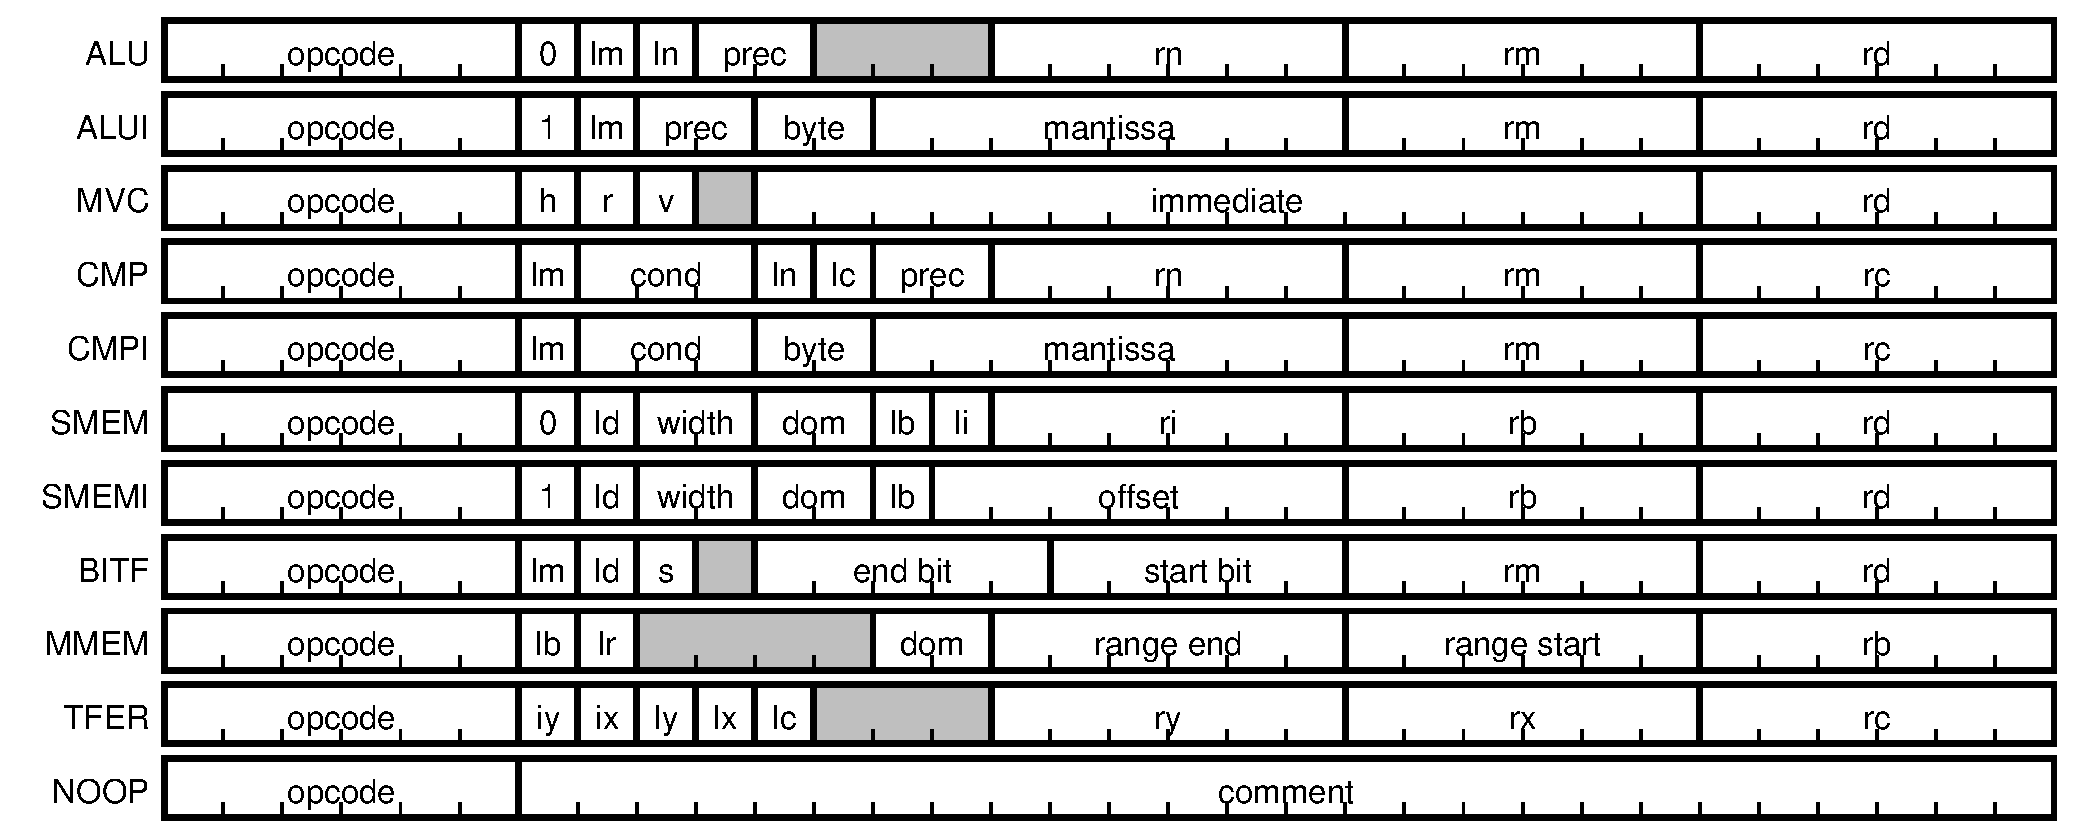
\includegraphics{aluform.eps}} \par}
\vspace{0.3cm}


\subsection{ALU and ALUI format instructions}

\newcommand{\decfmt}{
\begin{tabular}{ll}
\textit{Format} & \textit{Assembler syntax} \\[0.5ex]
}

\newcommand{\finfmt}{
\end{tabular}
}

\newcommand{\nex}[1]{$[$\textasciitilde$]$\texttt{#1}}

\subsubsection{mov}

\decfmt
\texttt{0000000.Npp...nnnnnn......dddddd} & \texttt{mov rd,\nex{rn}}\\
\texttt{0000001.ppbbiiiiiiii......dddddd} & \texttt{mov rd,\#imm}
\finfmt

Moves (copies) a value from one integer register to another, or from an immediate constant to a register. \texttt{rd} is the destination register, and \texttt{rn} is the source. If \texttt{N} is 1, \texttt{rn} is expired and becomes invalid.

If the immediate form is used, the immediate is calculated from the mantissa $i$ and byte number $b$, so that $b$ scales the mantissa by one of four values before putting it in \texttt{rd}.

\subsubsection{not}

\decfmt
\texttt{0000010.Npp...nnnnnn......dddddd} & \texttt{not rd,\nex{rn}}\\
\texttt{0000111.ppbbiiiiiiii......dddddd} & \texttt{not rd,\#imm}
\finfmt

Moves bitwise negation of \texttt{rn} or immediate into \texttt{rd}. If \texttt{N} is 1, \texttt{rn} is expired.

\subsubsection{lsl}

\decfmt
\texttt{0000100MNpp...nnnnnnmmmmmmdddddd} & \texttt{lsl rd,\nex{rm},\nex{rn}} \\
\texttt{0000101Mppbbiiiiiiiimmmmmmdddddd} & \texttt{lsl rd,\nex{rm},\#imm}
\finfmt

Logical shift left, \texttt{rd} gets \texttt{rm} shifted left \texttt{rn} or immediate places.

\subsubsection{lsr}

\decfmt
\texttt{0000110MNpp...nnnnnnmmmmmmdddddd} & \texttt{lsr rd,\nex{rm},\nex{rn}}\\
\texttt{0000111Mppbbiiiiiiiimmmmmmdddddd} & \texttt{lsr rd,\nex{rm},\#imm}
\finfmt

Logical shift right.

\subsubsection{asr}

\decfmt
\texttt{0001000MNpp...nnnnnnmmmmmmdddddd} & \texttt{asr rd,\nex{rm},\nex{rn}}\\
\texttt{0001001Mppbbiiiiiiiimmmmmmdddddd} & \texttt{asr rd,\nex{rm},\#imm}
\finfmt

Arithmetic shift right.

\subsubsection{ror}

\decfmt
\texttt{0001010MNpp...nnnnnnmmmmmmdddddd} & \texttt{ror rd,\nex{rm},\nex{rn}}\\
\texttt{0001011Mppbbiiiiiiiimmmmmmdddddd} & \texttt{ror rd,\nex{rm},\#imm}
\finfmt

Rotate right.

\subsubsection{and}

\decfmt
\texttt{0001100MNpp...nnnnnnmmmmmmdddddd} & \texttt{and rd,\nex{rm},\nex{rn}}\\
\texttt{0001101Mppbbiiiiiiiimmmmmmdddddd} & \texttt{and rd,\nex{rm},\#imm}
\finfmt

Bitwise AND.

\subsubsection{ior}

\decfmt
\texttt{0001110MNpp...nnnnnnmmmmmmdddddd} & \texttt{ior rd,\nex{rm},\nex{rn}}\\
\texttt{0001111Mppbbiiiiiiiimmmmmmdddddd} & \texttt{ior rd,\nex{rm},\#imm}
\finfmt

Bitwise inclusive OR.

\subsubsection{eor}

\decfmt
\texttt{0010000MNpp...nnnnnnmmmmmmdddddd} & \texttt{eor rd,\nex{rm},\nex{rn}} \\
\texttt{0010001Mppbbiiiiiiiimmmmmmdddddd} & \texttt{eor rd,\nex{rm},\#imm}
\finfmt

Bitwise exclusive OR.

\subsubsection{bic}

\decfmt
\texttt{0010010MNpp...nnnnnnmmmmmmdddddd} & \texttt{bic rd,\nex{rm},\nex{rn}} \\
\texttt{0010011Mppbbiiiiiiiimmmmmmdddddd} & \texttt{bic rd,\nex{rm},\#imm}
\finfmt

Bitwise AND NOT, \texttt{rd} becomes \texttt{rm} AND the bitwise compliment of \texttt{rn}.

\subsubsection{add}

\decfmt
\texttt{0010100MNpp...nnnnnnmmmmmmdddddd} & \texttt{add rd,\nex{rm},\nex{rn}} \\
\texttt{0010101Mppbbiiiiiiiimmmmmmdddddd} & \texttt{add rd,\nex{rm},\#imm}
\finfmt

Addition, modulo $2^{32}$. There is no carry-out or overflow, so in the rare cases these are needed they must be calculated manually.

\subsubsection{sub}

\decfmt
\texttt{0010110MNpp...nnnnnnmmmmmmdddddd} & \texttt{sub rd,\nex{rm},\nex{rn}} \\
\texttt{0010111Mppbbiiiiiiiimmmmmmdddddd} & \texttt{sub rd,\nex{rm},\#imm}
\finfmt

Subtraction modulo $2^{32}$, \texttt{rd} is set to the result of \texttt{rm} minus \texttt{rn} or immediate.

\subsubsection{rsb}

\decfmt
\texttt{0011000MNpp...nnnnnnmmmmmmdddddd} & \texttt{rsb rd,\nex{rm},\nex{rn}} \\
\texttt{0011001Mppbbiiiiiiiimmmmmmdddddd} & \texttt{rsb rd,\nex{rm},\#imm}
\finfmt

``Reverse'' subtraction modulo $2^{32}$, \texttt{rd} is set to the result of \texttt{rn} or immediate minus \texttt{rm}.

\subsubsection{mul}

\decfmt
\texttt{0011010MNpp...nnnnnnmmmmmmdddddd} & \texttt{mul rd,\nex{rm},\nex{rn}} \\
\texttt{0011011Mppbbiiiiiiiimmmmmmdddddd} & \texttt{mul rd,\nex{rm},\#imm}
\finfmt

Multiplication of two 32-bit values, yielding the low 32 bits of the result in \texttt{rd}. This is the same for signed and unsigned calculations. For the high part of the result use \texttt{mlh} or \texttt{umlh}.

\subsubsection{div}

\decfmt
\texttt{0011100MNpp...nnnnnnmmmmmmdddddd} & \texttt{div rd,\nex{rm},\nex{rn}} \\
\texttt{0011101Mppbbiiiiiiiimmmmmmdddddd} & \texttt{div rd,\nex{rm},\#imm}
\finfmt

Signed divide of two 32-bit values, yielding signed 32-bit result in \texttt{rd}.

\subsubsection{udiv}

\decfmt
\texttt{0011110MNpp...nnnnnnmmmmmmdddddd} & \texttt{udiv rd,\nex{rm},\nex{rn}} \\
\texttt{0011111Mppbbiiiiiiiimmmmmmdddddd} & \texttt{udiv rd,\nex{rm},\#imm}
\finfmt

Unsigned divide of two 32-bit values, yielding unsigned 32-bit result in \texttt{rd}.

\subsubsection{mod}

\decfmt
\texttt{0100000MNpp...nnnnnnmmmmmmdddddd} & \texttt{mod rd,\nex{rm},\nex{rn}} \\
\texttt{0100001Mppbbiiiiiiiimmmmmmdddddd} & \texttt{mod rd,\nex{rm},\#imm}
\finfmt

Signed modulus of two 32-bit values, yielding signed 32-bit result. The sign rules are as follows...

\subsubsection{umod}

\decfmt
\texttt{0100010MNpp...nnnnnnmmmmmmdddddd} & \texttt{umod rd,\nex{rm},\nex{rn}} \\
\texttt{0100011Mppbbiiiiiiiimmmmmmdddddd} & \texttt{umod rd,\nex{rm},\#imm}
\finfmt

Unsigned modulus of two 32-bit values, yielding unsigned 32-bit result. Result is never negative.

\subsubsection{mlh}

\decfmt
\texttt{0100100MNpp...nnnnnnmmmmmmdddddd} & \texttt{mlh rd,\nex{rm},\nex{rn}} \\
\texttt{0100101Mppbbiiiiiiiimmmmmmdddddd} & \texttt{mlh rd,\nex{rm},\#imm}
\finfmt

Register \texttt{rd} is set to the high 32 bits of the result of the signed multiplication of rm and rn or an immediate. Can be used for full 64-bit multiplication in conjunction with \texttt{mul}, or as constant reciprocal signed division.

\subsubsection{umlh}

\decfmt
\texttt{0100110MNpp...nnnnnnmmmmmmdddddd} & \texttt{umlh rd,\nex{rm},\nex{rn}} \\
\texttt{0100111Mppbbiiiiiiiimmmmmmdddddd} & \texttt{umlh rd,\nex{rm},\#imm}
\finfmt

Register \texttt{rd} is set to the high 32 bits of the result of the unsigned multiplication of rm and rn or an immediate. Can be used for full 64-bit unsigned multiplication in conjunction with \texttt{mul}, or as constant reciprocal unsigned division.

\subsection{MVC format instructions}

\subsubsection{mvc}

\decfmt
\texttt{01010000..iiiiiiiiiiiiiiiidddddd} & \texttt{mvc.l rd,\#0x....iiii}\\
\texttt{01010010..iiiiiiiiiiiiiiiidddddd} & \texttt{mvc.h rd,\#0xiiii....}\\
\texttt{010100010.iiiiiiiiiiiiiiiidddddd} & \texttt{mvc.el rd,\#0x0000iiii}\\
\texttt{010100110.iiiiiiiiiiiiiiiidddddd} & \texttt{mvc.eh rd,\#0xiiii0000}\\
\texttt{010100011.iiiiiiiiiiiiiiiidddddd} & \texttt{mvc.fl rd,\#0xFFFFiiii}\\
\texttt{010100111.iiiiiiiiiiiiiiiidddddd} & \texttt{mvc.fh rd,\#0xiiiiFFFF}\\
\finfmt

An instruction for getting a 16-bit immediate value into a register.
If the \texttt{h} bit is set, immediate is put into the high 16 bits of the
register \texttt{rd}, else the low 16 bits.

If the \texttt{r} (replace) bit is set, the ``other'' 16 bits are set to the
value of the \texttt{v} (value) bit, else they are left intact.

The \texttt{mvc} instruction can be used to load many common immediate values into a register, or can be used in pairs to load an arbitrary 32-bit value. The assembler works so that a pair of instructions can be used to load the address of a symbol into a register.

\textit{Example}

\texttt{mvc.el r5,\#\_foo\\
mvc.h r5,\#\_foo}

\subsection{CMP and CMPI format instructions}

\subsubsection{cmp}

\decfmt
\texttt{010101M000NCppnnnnnnmmmmmmcccccc} & \texttt{cmp.eq rc,\nex{rm},\nex{rn}} \\
\texttt{010110M000bbiiiiiiiimmmmmmcccccc} & \texttt{cmp.eq rc,\nex{rm},\#imm} \\
\texttt{010101M001NCppnnnnnnmmmmmmcccccc} & \texttt{cmp.ne rc,\nex{rm},\nex{rn}} \\
\texttt{010110M001bbiiiiiiiimmmmmmcccccc} & \texttt{cmp.ne rc,\nex{rm},\#imm} \\
\texttt{010101M010NCppnnnnnnmmmmmmcccccc} & \texttt{cmp.ge rc,\nex{rm},\nex{rn}} \\
\texttt{010110M010bbiiiiiiiimmmmmmcccccc} & \texttt{cmp.ge rc,\nex{rm},\#imm} \\
\texttt{010101M011NCppnnnnnnmmmmmmcccccc} & \texttt{cmp.gt rc,\nex{rm},\nex{rn}} \\
\texttt{010110M011bbiiiiiiiimmmmmmcccccc} & \texttt{cmp.gt rc,\nex{rm},\#imm} \\
\texttt{010101M100NCppnnnnnnmmmmmmcccccc} & \texttt{cmp.le rc,\nex{rm},\nex{rn}} \\
\texttt{010110M100bbiiiiiiiimmmmmmcccccc} & \texttt{cmp.le rc,\nex{rm},\#imm} \\
\texttt{010101M101NCppnnnnnnmmmmmmcccccc} & \texttt{cmp.lt rc,\nex{rm},\nex{rn}} \\
\texttt{010110M101bbiiiiiiiimmmmmmcccccc} & \texttt{cmp.lt rc,\nex{rm},\#imm} \\
\finfmt

Perform signed comparison of \texttt{rm} and \texttt{rn}, setting \texttt{rd} to `true' (-1, 0xFFFFFFFF) or `false' (0, 0x00000000) depending on the condition.

\subsubsection{ucmp}

\decfmt
\texttt{010111M010NCppnnnnnnmmmmmmcccccc} & \texttt{ucmp.ge rc,\nex{rm},\nex{rn}} \\
\texttt{011000M010bbiiiiiiiimmmmmmcccccc} & \texttt{ucmp.ge rc,\nex{rm},\#imm} \\
\texttt{010111M011NCppnnnnnnmmmmmmcccccc} & \texttt{ucmp.gt rc,\nex{rm},\nex{rn}} \\
\texttt{011000M011bbiiiiiiiimmmmmmcccccc} & \texttt{ucmp.gt rc,\nex{rm},\#imm} \\
\texttt{010111M100NCppnnnnnnmmmmmmcccccc} & \texttt{ucmp.le rc,\nex{rm},\nex{rn}} \\
\texttt{011000M100bbiiiiiiiimmmmmmcccccc} & \texttt{ucmp.le rc,\nex{rm},\#imm} \\
\texttt{010111M101NCppnnnnnnmmmmmmcccccc} & \texttt{ucmp.lt rc,\nex{rm},\nex{rn}} \\
\texttt{011000M101bbiiiiiiiimmmmmmcccccc} & \texttt{ucmp.lt rc,\nex{rm},\#imm} \\
\finfmt

Perform unsigned comparison of \texttt{rm} and \texttt{rn}, setting \texttt{rd} to `true' (-1, 0xFFFFFFFF) or `false' (0, 0x00000000) depending on the condition. There are also encodings for unsigned equality and inequality, but the meaning is the same as signed comparison so they are not listed.

\subsection{BITF format instructions}

\subsubsection{bfx}

\decfmt
\texttt{011001M.0.eeeeebbbbbmmmmmmdddddd} & \texttt{bfx rd,\nex{rm} <b,e>} \\
\texttt{011001M.1.eeeeebbbbbmmmmmmdddddd} & \texttt{bfx.s rd,\nex{rm} <b,e>}
\finfmt

Extracts a bitfield of \texttt{rm}, from bit \texttt{b} to bit \texttt{e} inclusive. The bitfield is shifted to start at the zeroth bit of \texttt{rd}. If \texttt{s} bit is true, the bitfield is sign-extended before putting it into \texttt{rd}.

This instruction is intended mainly as an aid to the dynamic optimiser, to allow it to decode instructions more efficiently. It may be simpler to omit it from a hardware implementation of DOP.

\subsection{SMEM and SMEMI format instructions}

\subsubsection{ldr}

\decfmt
\texttt{0110100.00xxBIiiiiiibbbbbbdddddd} & \texttt{ldr.b rd,@x[\nex{rb},\nex{ri}]} \\
\texttt{0110101.00xxBooooooobbbbbbdddddd} & \texttt{ldr.b rd,@x[\nex{rb},\#offset]} \\
\texttt{0110100.01xxBIiiiiiibbbbbbdddddd} & \texttt{ldr.h rd,@x[\nex{rb},\nex{ri}]} \\
\texttt{0110101.01xxBooooooobbbbbbdddddd} & \texttt{ldr.h rd,@x[\nex{rb},\#offset]} \\
\texttt{0110100.10xxBIiiiiiibbbbbbdddddd} & \texttt{ldr.w rd,@x[\nex{rb},\nex{ri}]} \\
\texttt{0110101.10xxBooooooobbbbbbdddddd} & \texttt{ldr.w rd,@x[\nex{rb},\#offset]}
\finfmt

Load a value from a memory location and put it in \texttt{rd}. The address is calculated as $\texttt{rb}+\texttt{ri}$, or as $\texttt{rb}+s*o$, where $s$ is 1 for byte loads, 2 for halfword loads and 4 for word loads, and $o$ is a sign-extended immediate.

\subsubsection{str}

\decfmt
\texttt{0110110D00xxBIiiiiiibbbbbbdddddd} & \texttt{str.b \nex{rd},@x[\nex{rb},\nex{ri}]} \\
\texttt{0110111D00xxBooooooobbbbbbdddddd} & \texttt{str.b \nex{rd},@x[\nex{rb},\#offset]} \\
\texttt{0110110D01xxBIiiiiiibbbbbbdddddd} & \texttt{str.h \nex{rd},@x[\nex{rb},\nex{ri}]} \\
\texttt{0110111D01xxBooooooobbbbbbdddddd} & \texttt{str.h \nex{rd},@x[\nex{rb},\#offset]} \\
\texttt{0110110D10xxBIiiiiiibbbbbbdddddd} & \texttt{str.w \nex{rd},@x[\nex{rb},\nex{ri}]} \\
\texttt{0110111D10xxBooooooobbbbbbdddddd} & \texttt{str.w \nex{rd},@x[\nex{rb},\#offset]}
\finfmt

Store value \texttt{rd} to a memory location. The address is calculated as $\texttt{rb}+\texttt{ri}$, or as $\texttt{rb}+s*o$, where $s$ is 1 for byte stores, 2 for halfword stores and 4 for word stores, and $o$ is a sign-extended immediate.

\subsection{MMEM format instructions}

\subsubsection{ldm}

\decfmt
\texttt{011100B.....xxeeeeeessssssbbbbbb} & \texttt{ldm \nex{rb},@x\{rs-re\}}
\finfmt

Load a contiguous range of registers from sequential memory addresses. Registers are transferred in order. The first load (of \texttt{rs}) comes from \texttt{rb}, and subsequent loads come from higher or lower addresses depending on the sign of $\texttt{e}-\texttt{s}$, such that increasing register numbers are always loaded from increasing memory locations, and vice versa.

\subsubsection{stm}

\decfmt
\texttt{011101BR....xxeeeeeessssssbbbbbb} & \texttt{stm \nex{rb},@x\nex{\{rs-re\}}}
\finfmt

Store a contiguous range of registers to sequential memory addresses. Registers are transferred in order. The first store (of \texttt{rs}) goes to \texttt{rb}, and subsequent stores go to higher or lower addresses depending on the sign of $\texttt{e}-\texttt{s}$, such that increasing register numbers are always stored at increasing memory locations, and vice versa. If the \texttt{R} bit is 1, the entire range of registers is expired after the store.

\subsection{NOOP format instructions}

\subsubsection{swi}

\decfmt
\texttt{011110cccccccccccccccccccccccccc} & \texttt{swi \#comment}
\finfmt

(Eventually) trap to supervisor mode, branch through a SWI vector (to OS). Currently used to fake a microscopic `operating system'.

\subsubsection{ldx, ldy, ldz}

\decfmt
\texttt{111101iiiiiiiiiiiiiiiiiiiiiiiiii} & \texttt{ldx \#imm} \\
\texttt{111110iiiiiiiiiiiiiiiiiiiiiiiiii} & \texttt{ldy \#imm} \\
\texttt{111111iiiiiiiiiiiiiiiiiiiiiiiiii} & \texttt{ldz \#imm}
\finfmt

Load the internal 26-bit X, Y and Z registers with immediate value. These registers are used for control flow. These instructions are generated automatically by the assembler if the immediate forms of \texttt{TFER} format instructions are used, so they need not (and must not) be written explicitly. They may be recoded in a more efficient form later on.

\subsection{ALU and ALUI format float instructions}

\subsubsection{movf}

\decfmt
\texttt{0111110.N00...nnnnnn......dddddd} & \texttt{movf.s fd,\nex{fn}} \\
\texttt{0111110.N01...nnnnnn......dddddd} & \texttt{movf.d fd,\nex{fn}} \\
\texttt{0111111.00bbiiiiiiii......dddddd} & \texttt{movf.s fd,\#imm} \\
\texttt{0111111.01bbiiiiiiii......dddddd} & \texttt{movf.d fd,\#imm} \\
\finfmt

Moves (copies) \texttt{fn} or immediate to \texttt{fd}, casting to the given precision (IEEE754 single or double). The immediate is an integer, and is converted to a float before putting it into \texttt{fd}. Most floating-point constants are not representable, and thus must be loaded from memory.

\subsubsection{negf}

\decfmt
\texttt{1000000.N00...nnnnnn......dddddd} & \texttt{negf.s fd,\nex{fn}} \\
\texttt{1000000.N01...nnnnnn......dddddd} & \texttt{negf.d fd,\nex{fn}} \\
\texttt{1000001.00bbiiiiiiii......dddddd} & \texttt{negf.s fd,\#imm} \\
\texttt{1000001.01bbiiiiiiii......dddddd} & \texttt{negf.d fd,\#imm} \\
\finfmt

Negates \texttt{fn} or immediate, and puts result in \texttt{fd} with given precision.

\subsubsection{absf}

\decfmt
\texttt{1000010.N00...nnnnnn......dddddd} & \texttt{absf.s fd,\nex{fn}} \\
\texttt{1000010.N01...nnnnnn......dddddd} & \texttt{absf.d fd,\nex{fn}} \\
\texttt{1000011.00bbiiiiiiii......dddddd} & \texttt{absf.s fd,\#imm} \\
\texttt{1000011.01bbiiiiiiii......dddddd} & \texttt{absf.d fd,\#imm} \\
\finfmt

Finds absolute value of \texttt{fn} or immediate, and puts result in \texttt{fd} with given precision.

\subsubsection{sqrf}

\decfmt
\texttt{1000100.N00...nnnnnn......dddddd} & \texttt{sqrf.s fd,\nex{fn}} \\
\texttt{1000100.N01...nnnnnn......dddddd} & \texttt{sqrf.d fd,\nex{fn}} \\
\texttt{1000101.00bbiiiiiiii......dddddd} & \texttt{sqrf.s fd,\#imm} \\
\texttt{1000101.01bbiiiiiiii......dddddd} & \texttt{sqrf.d fd,\#imm} \\
\finfmt

Finds square root of \texttt{fn} or immediate with given precision, and puts result in \texttt{fd}.

\subsubsection{fltf}

\decfmt
\texttt{1000110.N00...nnnnnn......dddddd} & \texttt{fltf.s fd,\nex{rn}} \\
\texttt{1000110.N01...nnnnnn......dddddd} & \texttt{fltf.d fd,\nex{rn}} \\
\finfmt

Finds floating-point value of integer register, and puts result in \texttt{fd} with given precision.

\subsubsection{fixf}

\decfmt
\texttt{1001000.N00...nnnnnn......dddddd} & \texttt{fixf.s rd,\nex{fn}} \\
\texttt{1001000.N01...nnnnnn......dddddd} & \texttt{fixf.d rd,\nex{fn}} \\
\finfmt

Finds largest integer not greater than \texttt{fn}, and puts result in (integer) register \texttt{rd}.

\subsubsection{addf}

\decfmt
\texttt{1001010MN00...nnnnnnmmmmmmdddddd} & \texttt{addf.s fd,\nex{fm},\nex{fn}} \\
\texttt{1001010MN01...nnnnnnmmmmmmdddddd} & \texttt{addf.d fd,\nex{fm},\nex{fn}} \\
\texttt{1001011M00bbiiiiiiiimmmmmmdddddd} & \texttt{addf.s fd,\nex{fm},\#imm} \\
\texttt{1001011M01bbiiiiiiiimmmmmmdddddd} & \texttt{addf.d fd,\nex{fm},\#imm}
\finfmt

Adds \texttt{fm} to \texttt{fn} or immediate, and puts result in \texttt{fd} with given precision.

\subsubsection{subf}

\decfmt
\texttt{1001100MN00...nnnnnnmmmmmmdddddd} & \texttt{subf.s fd,\nex{fm},\nex{fn}} \\
\texttt{1001100MN01...nnnnnnmmmmmmdddddd} & \texttt{subf.d fd,\nex{fm},\nex{fn}} \\
\texttt{1001101M00bbiiiiiiiimmmmmmdddddd} & \texttt{subf.s fd,\nex{fm},\#imm} \\
\texttt{1001101M01bbiiiiiiiimmmmmmdddddd} & \texttt{subf.d fd,\nex{fm},\#imm}
\finfmt

Subtracts \texttt{fn} or immediate from \texttt{fm}, and puts result in \texttt{fd} with given precision.

\subsubsection{mulf}

\decfmt
\texttt{1001110MN00...nnnnnnmmmmmmdddddd} & \texttt{mulf.s fd,\nex{fm},\nex{fn}} \\
\texttt{1001110MN01...nnnnnnmmmmmmdddddd} & \texttt{mulf.d fd,\nex{fm},\nex{fn}} \\
\texttt{1001111M00bbiiiiiiiimmmmmmdddddd} & \texttt{mulf.s fd,\nex{fm},\#imm} \\
\texttt{1001111M01bbiiiiiiiimmmmmmdddddd} & \texttt{mulf.d fd,\nex{fm},\#imm}
\finfmt

Multiplies \texttt{fn} or immediate and \texttt{fm}, and puts result in \texttt{fd} with given precision.

\subsubsection{divf}

\decfmt
\texttt{1010000MN00...nnnnnnmmmmmmdddddd} & \texttt{divf.s fd,\nex{fm},\nex{fn}} \\
\texttt{1010000MN01...nnnnnnmmmmmmdddddd} & \texttt{divf.d fd,\nex{fm},\nex{fn}} \\
\texttt{1010001M00bbiiiiiiiimmmmmmdddddd} & \texttt{divf.s fd,\nex{fm},\#imm} \\
\texttt{1010001M01bbiiiiiiiimmmmmmdddddd} & \texttt{divf.d fd,\nex{fm},\#imm}
\finfmt

Divides \texttt{fm} by \texttt{fn} or immediate, and puts result in \texttt{fd} with given precision.

\subsection{CMP format float instructions}

\subsubsection{cmpf}

\decfmt
\texttt{101001M000N.00nnnnnnmmmmmmcccccc} & \texttt{cmpf.eq.s rc,\nex{fm},\nex{fn}} \\
\texttt{101001M000N.01nnnnnnmmmmmmcccccc} & \texttt{cmpf.eq.d rc,\nex{fm},\nex{fn}} \\
\texttt{101001M001N.00nnnnnnmmmmmmcccccc} & \texttt{cmpf.ne.s rc,\nex{fm},\nex{fn}} \\
\texttt{101001M001N.01nnnnnnmmmmmmcccccc} & \texttt{cmpf.ne.d rc,\nex{fm},\nex{fn}} \\
\texttt{101001M010N.00nnnnnnmmmmmmcccccc} & \texttt{cmpf.ge.s rc,\nex{fm},\nex{fn}} \\
\texttt{101001M010N.01nnnnnnmmmmmmcccccc} & \texttt{cmpf.ge.d rc,\nex{fm},\nex{fn}} \\
\texttt{101001M011N.00nnnnnnmmmmmmcccccc} & \texttt{cmpf.gt.s rc,\nex{fm},\nex{fn}} \\
\texttt{101001M011N.01nnnnnnmmmmmmcccccc} & \texttt{cmpf.gt.d rc,\nex{fm},\nex{fn}} \\
\texttt{101001M100N.00nnnnnnmmmmmmcccccc} & \texttt{cmpf.le.s rc,\nex{fm},\nex{fn}} \\
\texttt{101001M100N.01nnnnnnmmmmmmcccccc} & \texttt{cmpf.le.d rc,\nex{fm},\nex{fn}} \\
\texttt{101001M101N.00nnnnnnmmmmmmcccccc} & \texttt{cmpf.lt.s rc,\nex{fm},\nex{fn}} \\
\texttt{101001M101N.01nnnnnnmmmmmmcccccc} & \texttt{cmpf.lt.d rc,\nex{fm},\nex{fn}}
\finfmt

Floating-point comparison of \texttt{fm} and \texttt{fn} with given precision, putting true (-1) or false (0) result in integer register \texttt{rc} depending on the condition.

Several important floating-point comparisons are missing, including the ``unordered'' test. What does that mean exactly? Something to do with NaNs and/or infinities I think.

\subsection{SMEM and SMEMI format float instructions}

\subsubsection{ldf}

\decfmt
\texttt{1010100.00xxBIiiiiiibbbbbbdddddd} & \texttt{ldf.s fd,@x[\nex{rb},\nex{ri}]} \\
\texttt{1010101.00xxBooooooobbbbbbdddddd} & \texttt{ldf.s fd,@x[\nex{rb},\#offset]} \\
\texttt{1010100.01xxBIiiiiiibbbbbbdddddd} & \texttt{ldf.d fd,@x[\nex{rb},\nex{ri}]} \\
\texttt{1010101.01xxBooooooobbbbbbdddddd} & \texttt{ldf.d fd,@x[\nex{rb},\#offset]} \\
\finfmt

Load a value from a memory location and put it in \texttt{fd}. The address is calculated as $\texttt{rb}+\texttt{ri}$, or as $\texttt{rb}+4*o$, where $o$ is a sign-extended immediate. Four bytes are loaded for single-precision, eight bytes for double-precision.

\subsubsection{ldf}

\decfmt
\texttt{1010110D00xxBIiiiiiibbbbbbdddddd} & \texttt{stf.s \nex{fd},@x[\nex{rb},\nex{ri}]} \\
\texttt{1010111D00xxBooooooobbbbbbdddddd} & \texttt{stf.s \nex{fd},@x[\nex{rb},\#offset]} \\
\texttt{1010110D01xxBIiiiiiibbbbbbdddddd} & \texttt{stf.d \nex{fd},@x[\nex{rb},\nex{ri}]} \\
\texttt{1010111D01xxBooooooobbbbbbdddddd} & \texttt{stf.d \nex{fd},@x[\nex{rb},\#offset]} \\
\finfmt

Store \texttt{fd} to a memory location. The address is calculated as $\texttt{rb}+\texttt{ri}$, or as $\texttt{rb}+4*o$, where $o$ is a sign-extended immediate.

\subsection{MMEM format float instructions}

\subsubsection{ldmf}

\decfmt
\texttt{101100B.....xxeeeeeessssssbbbbbb} & \texttt{ldmf \nex{rb},@x\{fs-fe\}}
\finfmt

Load a contiguous range of double-precision floating point registers from sequential memory addresses. Registers are transferred in order. The first load (of \texttt{fs}) comes from \texttt{rb}, and subsequent loads come from higher or lower addresses depending on the sign of $\texttt{e}-\texttt{s}$, such that increasing register numbers are always loaded from increasing memory locations, and vice versa.

\subsubsection{stmf}

\decfmt
\texttt{101101BR....xxeeeeeessssssbbbbbb} & \texttt{stmf \nex{rb},@x\nex{\{fs-fe\}}}
\finfmt

Store a contiguous range of double-precision floating-point registers to sequential memory addresses. Registers are transferred in order. The first store (of \texttt{fs}) goes to \texttt{rb}, and subsequent stores go to higher or lower addresses depending on the sign of $\texttt{e}-\texttt{s}$, such that increasing register numbers are always stored at increasing memory locations, and vice versa. If the \texttt{R} bit is 1, the entire range of registers is expired after the store.

\subsection{TFER format instructions}

\subsubsection{trapz}

\decfmt
\texttt{10111000.ZC.........zzzzzzcccccc} & \texttt{trapz \nex{rc},\nex{rz}} \\
\texttt{10111001..C.........zzzzzzcccccc} & \texttt{trapz \nex{rc},\#hi\_z} \\
\finfmt

Trap on zero. If register \texttt{rc} is zero, jump to location Z, formed from register \texttt{rz} or immediate \texttt{hi\_z} and bottom 26 bits of internal Z register.

\subsubsection{trapn}

\decfmt
\texttt{10111100.ZC.........zzzzzzcccccc} & \texttt{trapn \nex{rc},\nex{rz}} \\
\texttt{10111101..C.........zzzzzzcccccc} & \texttt{trapn \nex{rc},\#hi\_z} \\
\finfmt

Trap on nonzero. If register \texttt{rc} is nonzero, jump to location Z, formed from register \texttt{rz} or immediate \texttt{hi\_z} and bottom 26 bits of internal Z register.

\subsubsection{cbr}

\decfmt
\texttt{11000000YXC...yyyyyyxxxxxxcccccc} & \texttt{cbr \nex{rc},\nex{rx},\nex{ry}} \\
\texttt{11000001Y.C...yyyyyyxxxxxxcccccc} & \texttt{cbr \nex{rc},\#hi\_x,\nex{ry}} \\
\texttt{11000010.XC...yyyyyyxxxxxxcccccc} & \texttt{cbr \nex{rc},\nex{rx},\#hi\_y} \\
\texttt{11000011..C...yyyyyyxxxxxxcccccc} & \texttt{cbr \nex{rc},\#hi\_x,\#hi\_y}
\finfmt

Conditional branch. If register \texttt{rc} is nonzero, jump to location X, else jump to location Y\@. X and Y are formed from registers \texttt{rx} and \texttt{ry}, or from immediates \texttt{hi\_x} and \texttt{hi\_y} and bottom 26 bits of the internal X and Y registers.

\subsubsection{call}

\decfmt
\texttt{11000100YX....yyyyyyxxxxxx......} & \texttt{call \nex{rx},\nex{ry}} \\
\texttt{11000101Y.....yyyyyyxxxxxx......} & \texttt{call \#hi\_x,\nex{ry}} \\
\texttt{11000110.X....yyyyyyxxxxxx......} & \texttt{call \nex{rx},\#hi\_y} \\
\texttt{11000111......yyyyyyxxxxxx......} & \texttt{call \#hi\_x,\#hi\_y}
\finfmt

The call instruction is used to invoke subroutines. Copies location Y to \texttt{r62}, then transfers control to location X\@. X and Y are formed from registers \texttt{rx} and \texttt{ry}, or from immediates \texttt{hi\_x} and \texttt{hi\_y} and bottom 26 bits of the internal X and Y registers.

\subsubsection{jump}

\decfmt
\texttt{110010.0.X..........xxxxxx......} & \texttt{jump \nex{rx}} \\
\texttt{110010.1............xxxxxx......} & \texttt{jump \#hi\_x}
\finfmt

Unconditional jump to location X, formed as above.

\subsubsection{ret}

\decfmt
\texttt{110011..........................} & \texttt{ret}
\finfmt

Unconditional jump to \texttt{r62}, used specifically to return to the calling context of a subroutine.

If it is desired to return to another location (for example in the implementation of coroutines), a \texttt{jump} through a register should be used instead (\texttt{r62} or otherwise), as the optimiser may make use of the ``stack semantics'' of normal function calls at some point.
